\documentclass[11pt,a4paper]{article}

% Packages
\usepackage{amsmath,amssymb,amsfonts}
\usepackage{graphicx}
\usepackage{xcolor}
\usepackage{hyperref}
\usepackage{booktabs}
\usepackage{algorithm}
\usepackage{algpseudocode}
\usepackage{tikz}
\usepackage{chemformula}
\usepackage[margin=1in]{geometry}
\usepackage{fontspec}
\usepackage{listings}
\usepackage{microtype}
\usepackage{mhchem}
\usepackage{tabularx}

% Custom colors
\definecolor{deepblue}{RGB}{0,0,120}
\definecolor{midgreen}{RGB}{0,120,0}
\definecolor{darkred}{RGB}{120,0,0}
\definecolor{codecolor}{RGB}{240,240,240}

% Setup code listings
\lstset{
  backgroundcolor=\color{codecolor},
  basicstyle=\footnotesize\ttfamily,
  breaklines=true,
  captionpos=b,
  keepspaces=true,
  columns=flexible,
  tabsize=2,
  frame=single,
  numbers=none,
  numberstyle=\tiny\color{gray},
  keywordstyle=\color{blue},
  commentstyle=\color{darkred},
  stringstyle=\color{midgreen}
}

% Hyperref setup
\hypersetup{
    colorlinks=true,
    linkcolor=blue,
    filecolor=magenta,
    urlcolor=cyan,
}

% Title information
\title{\Large\textbf{AI-Driven Design of Fridge-Free Insulin Delivery Patches:\\An Active Learning Framework Integrating LLMs and MD Simulations}}
\author{BioMaterials AI Research Group}
\date{\today}

\begin{document}

\maketitle

\begin{abstract}
I introduce a computational framework for the discovery and optimization of novel materials for fridge-free insulin delivery patches. This system leverages large language models (LLMs) for scientific literature mining, deep generative models for material design, and molecular dynamics (MD) simulations to evaluate critical properties such as thermal stability, insulin encapsulation efficiency, controlled release kinetics, and biocompatibility. Our active learning approach iteratively refines material candidates through feedback loops between these components, hopefully accelerating discovery of suitable materials that can maintain insulin stability without refrigeration.
\end{abstract}

\section{System Architecture}

Our active learning framework consists of three integrated components:

\begin{figure}[h]
\centering
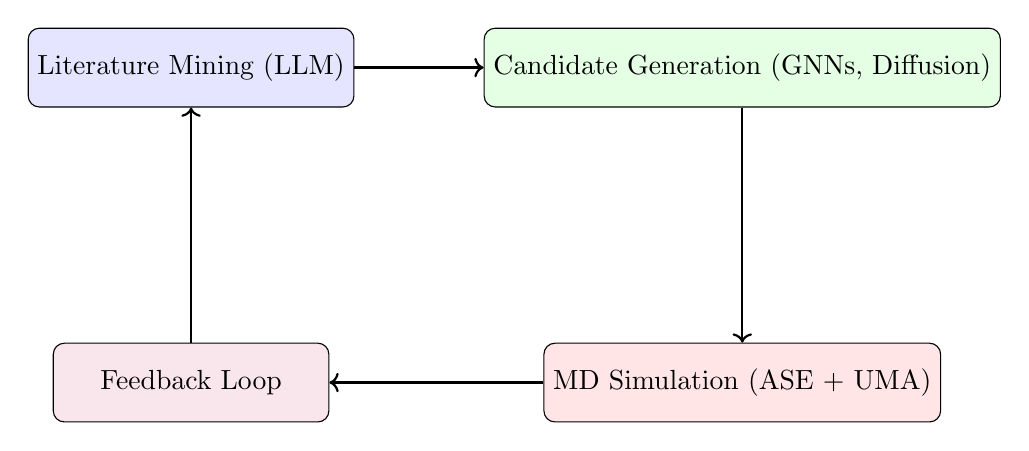
\begin{tikzpicture}[node distance=3cm]
\node (llm) [rectangle, rounded corners, draw, fill=blue!10, minimum width=3.5cm, minimum height=1cm] {Literature Mining (LLM)};
\node (select) [rectangle, rounded corners, draw, fill=green!10, minimum width=3.5cm, minimum height=1cm, right of=llm, xshift=4cm] {Candidate Generation (GNNs, Diffusion)};
\node (md) [rectangle, rounded corners, draw, fill=red!10, minimum width=3.5cm, minimum height=1cm, below of=select, yshift=-1cm] {MD Simulation (ASE + UMA)};
\node (feedback) [rectangle, rounded corners, draw, fill=purple!10, minimum width=3.5cm, minimum height=1cm, left of=md, xshift=-4cm] {Feedback Loop};
\draw[->, thick] (llm) -- (select);
\draw[->, thick] (select) -- (md);
\draw[->, thick] (md) -- (feedback);
\draw[->, thick] (feedback) -- (llm);
\end{tikzpicture}
\caption{Active learning workflow for fridge-free insulin patch material discovery. The loop begins with literature mining (LLM)}
\label{fig:workflow}
\end{figure}

\subsection{LLM-Guided Literature Mining}

Our framework begins by systematically extracting relevant information about potential materials for insulin delivery from the scientific literature. We utilize large language models (open source and local, for the prototype) to:

\begin{itemize}
    \item Identify existing materials (polymers, hydrogels, nanomaterials) used for protein stabilization
    \item Extract reported thermal stability properties and insulin compatibility
    \item Gather information on transdermal delivery efficacy
    \item Identify structural features that contribute to protein stabilization
\end{itemize}

When prompted with specific queries about materials for insulin delivery, the LLM returns structured data including:

\begin{itemize}
    \item Material composition and structure
    \item Reported insulin stability duration at various temperatures
    \item Biocompatibility data
    \item Release kinetics and delivery efficiency
    \item Mechanism of stabilization (e.g., hydrogen bonding, hydrophobic interactions)
\end{itemize}

Sample prompt:

\begin{lstlisting}
Identify hydrogels and polymers reported in literature with demonstrated 
thermal stabilization of proteins and peptides at temperatures between 
25-40°C. For each material, extract the chemical composition, stabilization 
mechanism, reported stability period, biocompatibility data, and any 
information on controlled release properties.
\end{lstlisting}

\subsection{Deep Learning for Candidate Material Generation}

From the LLM-identified materials in the literature, we generate novel molecular structures using generative modeling to modify these materials into specific hypothetical candidates with optimized properties.

Our generative approach can employ (they exist online):

\begin{itemize}
    \item Graph Neural Networks (GNNs) for polymer and hydrogel structure modifications
    \item Diffusion models for generating novel material compositions
    \item Variational autoencoders (VAEs) for exploring the chemical space around promising candidates
\end{itemize}

These models are specifically trained to:

\begin{itemize}
    \item Modify side chains while preserving backbone structure
    \item Adjust crosslinking density and patterns
    \item Optimize hydrophilic/hydrophobic balance
    \item Incorporate motifs identified as beneficial through literature mining
\end{itemize}

For example, if the LLM identifies PEG-based hydrogels as promising materials, our generative models can create dozens of variants with systematically modified side chains to optimize insulin interactions.

\section{Material Property Evaluation via MD Simulations with UMA}

For each candidate material, we conduct molecular dynamics simulations to evaluate critical properties for insulin delivery patches. A key innovation in our approach is the adoption of Meta FAIR's Universal Model for Atoms (UMA) force field integrated with the Atomic Simulation Environment (ASE).

\subsection{UMA Force Field Integration}

Traditional MD simulations face significant challenges when evaluating novel materials due to the lack of reliable force field parameters. We address this limitation by implementing the Universal Model for Atoms (UMA) recently released by Meta FAIR:

\begin{itemize}
    \item UMA provides universal force field parameters for arbitrary molecular systems
    \item It employs machine learning models trained on massive quantum mechanical calculations (over 100 million molecular configurations)
    \item The model captures interactions at multiple scales, from atomic to molecular
    \item UMA's transferability makes it ideal for novel materials without established parameters
    \item UMA can perform calculations up to 10,000 times faster than traditional Density Functional Theory
\end{itemize}

This approach allows us to simulate novel materials generated by our AI models without the traditional bottleneck of force field parameterization, dramatically accelerating our discovery pipeline.

\subsection{ASE-UMA MD Simulation Protocol}

Our simulation workflow utilizes the Atomic Simulation Environment (ASE) for interfacing with UMA:

\begin{algorithm}
\caption{Insulin-Material MD Evaluation Pipeline with ASE-UMA}
\begin{algorithmic}[1]
\State \textbf{Input:} Candidate material structure $M$, insulin model
\State Generate material-insulin complex structure in ASE
\State Apply UMA force field through FAIRChemCalculator
\State Perform energy minimization with ASE optimizers
\State Run MD simulation with ASE molecular dynamics modules
\State Calculate: thermal stability, insulin conformation, diffusion rates
\State Simulate water penetration and insulin release
\State \textbf{Return:} Stability and release metrics with uncertainty estimates
\end{algorithmic}
\end{algorithm}

We evaluate four critical properties for insulin delivery patches:

\begin{table}[h]
\centering
\begin{tabularx}{\linewidth}{XlX}
\toprule
\textbf{Property} & \textbf{Simulation Type} & \textbf{Analysis Method} \\
\midrule
Thermal stability & High-T NPT & RMSD of material structure \\
Insulin protection & NPT with insulin & Protein secondary structure analysis \\
Water penetration & NPT with water contact & Diffusion coefficient calculation \\
Release kinetics & Non-equilibrium MD & Steered MD with PMF calculation \\
\bottomrule
\end{tabularx}
\caption{MD simulation protocols for insulin patch material properties}
\label{tab:md_protocols}
\end{table}

\section{Dynamic LLM Feedback Loop}

A critical aspect of our system is the continuous integration of LLMs within the active learning cycle. The LLM doesn't simply function as a one-time literature extraction tool but remains an active component throughout the discovery process. We achieve this through dynamic prompt engineering.

\subsection{Prompt Template Architecture}

We developed a template-based prompting system that evolves with each iteration:

\begin{lstlisting}
# Base Template for Insulin Material Search
INPUT:
- [Iteration Number]: {iteration}
- [Previous High-performing Materials]: {top_candidates}
- [Observed Stability Mechanisms]: {stability_mechanisms}
- [Target Properties to Optimize]: {target_properties}
- [Current Performance Limitations]: {limitations}

OUTPUT REQUEST:
Identify {num_candidates} materials with these characteristics:
1. {Required_property_1} [with specific threshold values]
2. {Required_property_2} [with specific threshold values]
3. Must contain or leverage {beneficial_structural_motif}
4. Exclude materials with {problematic_features}

For each candidate, provide:
1. Complete chemical composition
2. Structure information (backbone, side chains, crosslinking)
3. Predicted stabilization mechanism
4. Literature references supporting your suggestions
\end{lstlisting}

After each iteration of MD simulations, we programmatically populate this template with new insights:

\begin{itemize}
    \item \{top\_candidates\} lists the highest-performing materials from previous iterations
    \item \{stability\_mechanisms\} includes specific molecular interactions identified through MD
    \item \{beneficial\_structural\_motif\} highlights structural features correlated with insulin stability
    \item \{problematic\_features\} flags material characteristics that led to poor performance
\end{itemize}

\subsection{Dynamic Prompt Evolution Example}

To illustrate how prompts evolve throughout the active learning process, consider this progression for hydrogel material discovery:

\textbf{Iteration 1 (Initial Exploration):}
\begin{lstlisting}
Identify hydrogels and polymers reported in literature for protein 
stabilization. For each material, extract the chemical composition, 
reported stability mechanism, biocompatibility data, and any information 
on controlled release properties.
\end{lstlisting}

\textbf{Iteration 3 (After Initial MD Insights):}
\begin{lstlisting}
Based on our MD simulations, we found that PEG-based hydrogels with 
carboxylic acid side chains showed promising insulin stabilization 
through hydrogen bonding with insulin B-chain residues. 

Identify 15 additional materials that:
1. Contain similar hydrogen-bonding capabilities
2. Offer varied hydrophobic/hydrophilic balance
3. Maintain stability at 37°C

Include specific side chain configurations and crosslinking strategies.
\end{lstlisting}

\textbf{Iteration 6 (More Targeted Exploration):}
\begin{lstlisting}
Our simulations revealed that hydrogels with alternating hydrophilic/
hydrophobic domains and specific spacing (4-6 Å) between binding sites 
demonstrate superior insulin conformation preservation. Materials with 
solely PEG-based backbones showed water retention issues affecting 
release kinetics.

Identify 10 new materials that:
1. Maintain the beneficial alternating domain structure
2. Incorporate zwitterionic elements for improved water management
3. Explore non-PEG backbones that maintain required spacing
4. Avoid materials with high crystallinity (>35%) which correlated 
   with poor insulin release

For each suggestion, detail the expected molecular interactions with 
insulin B9-B19 residues, which our model identified as critical 
stabilization sites.
\end{lstlisting}

This continuous refinement of prompts allows the LLM to perform increasingly targeted literature mining based on the accumulated knowledge from previous iterations.

\subsection{Integration with Generative Models}

While the LLM component identifies candidate materials from existing literature, our generative models focus on designing novel variations:

\begin{itemize}
    \item LLM identifies promising base materials and stabilization principles
    \item Generative models (GNNs, diffusion models) create systematic modifications:
    \begin{itemize}
        \item Side chain substitutions
        \item Backbone modifications
        \item Crosslinking pattern variations
        \item Incorporation of identified beneficial motifs
    \end{itemize}
    \item MD simulations with UMA evaluate both literature-derived and AI-generated candidates
    \item Results feed back to both LLM prompts and generative model conditioning
\end{itemize}

This dual approach allows us to leverage existing scientific knowledge through LLMs while exploring novel chemical spaces through generative models. The LLM component helps interpret simulation results and guides the generative models toward promising regions of the material design space.

\end{document}